\documentclass[12pt]{article}
\usepackage[left=2cm, right=2cm, top=2cm]{geometry}
\usepackage[utf8]{inputenc} 
\usepackage{graphicx} % to include images
\usepackage{amsmath} % For math mode
\usepackage{caption} % For captions
\usepackage{subcaption} % To use caption while using mini page
\usepackage{amssymb} % To use math symbols
\usepackage{multirow} %To combine multiple rows in a table
\usepackage[table]{xcolor} %To color rows / columns in table
\usepackage{titling} %To vertically center the title page
\usepackage{hyperref} %for URL
\usepackage[none]{hyphenat} %To remove hyphen
\usepackage{caption} %For table captions


%----------------------------MATLAB TEMPLATE -------------------------------------
\usepackage{listings}
\usepackage{color} %red, green, blue, yellow, cyan, magenta, black, white
\definecolor{mygreen}{RGB}{28,172,0} % color values Red, Green, Blue
\definecolor{mylilas}{RGB}{170,55,241}
%-----------------------------------------------------------------------------------------

\title{MATH 8650\\ Advanced Data Structures \\ 
	Term Project \\ Optimization of Bellman Ford Algorithm}
\author{Vivek Koodli Udupa (C12768888) \\ Sai Harsha Nagabothu (C11086803) } 
\date{November - 30, 2018 }

%To make the title page center vertically centered
\renewcommand\maketitlehooka{\null\mbox{}\vfill}
\renewcommand\maketitlehookd{\vfill\null}

\begin{document}

%Displaying Title
\begin{titlepage}
\maketitle
\pagenumbering{gobble}% Remove page numbers (and reset to 1)
\end{titlepage}
\pagenumbering{arabic}% Arabic page numbers (and reset to 1)


%Begin of Report
\begin{center}
	\section*{Abstract}
\end{center}

Dijkstra's and Bellman Ford algorithms are two of the popular algorithms used for path finding. Though Dijkstra's outperforms Bellman Ford, it does not work in the presence of negative edge weight cycle. To get the best of both algorithms, Shortest Path Faster Algorithm(SPFA) is used. This report presents the comparison study of the above mentioned algorithms. \\

\section{Introduction}
This report considers the problem of shortest path finding. Shortest path is the minimum cost between two vertices in a  given graph. The common algorithms used to find the shortest paths are Dijkstra, A*, Floyd-Warshall and Bellman Ford. Bellman Ford algorithm works with negative edge weights and it detects negative cycles in the given graph. Detecting negative cycles are important as they can cause the algorithm to run into an infinite loop. Edge weights are not only restricted to represent length, but can also represent time, money and negative costs like loss. \\

Consider the example of traffic congestion on a map. Here the weights represent traffic conditions in the map. More unfavorable conditions results is more negative weights. In such cases, Bellman Ford algorithm is considered. In order to optimize the performance of Bellman Ford algorithm, SPFA is considered. \\ 

Shortest Path Faster Algorithm (SPFA) is an optimization of Bellman Ford Algorithm which computes single-source shortest path in a weighted directed graph. Though the worst-case complexity of SPFA is same as Bellman Ford, it performs better on practical random graphs. \\

In this report, we do a comparison study between Bellman Ford, Dijkstra's and several versions of SPFA which are SPFA - FIFO, SPFA - LIFO and SPFA - PAPE. \\

\section{Implementation}
\label{sec:impl}
This section describes the implementation of Bellman Ford and the three versions of SPFA algorithms. \\

The input to the Bellman Ford Algorithm is (G, src), where $G = (V, E)$ is a directed graph with V vertices and E Edges. src $\in$ V is the source node and the algorithm finds the shortest path from src to all other nodes. \\  

The following steps are considered while implementing the Bellman Ford Algorithm:
\begin{enumerate}
	\item Create a distance array, dist[] and initialize it to infinity for all nodes and zero for source. 
	
	\item Perform relaxation of nodes for V - 1 times. This finds the shortest distances. 
	
	\item Perform negative cycle check by doing one more relaxation. 
	
	\item Display the results.  
\end{enumerate}

\subsection{Negative Cycle Check}
For a given source node, Bellman Ford algorithm first calculates the shortest distance which has at-most one edge in the path. Then, it calculates shortest path with at-most two edges, and so on. After V - 1 iterations, shortest distance to all the vertices in the graph will be calculated. \\ 
Another shorter distance is after the $V - 1^{th}$ iteration indicates the presence of a Negative Cycle. The algorithm can be stopped here otherwise it will fall into an infinite loop. \\

\subsection{Node Relaxation}
Relaxation is the most important step in Bellman-Ford. It is what increases the accuracy of the distance to any given vertex. Relaxation works by continuously shortening the calculated distance between vertices comparing that distance with other known distances. \\

The distance of the current node is compared with the sum of the weight(w) of the edge and the distance of the node connected to the edge. If the sum is lesser than then distance of the current node, then the current node distance is updated. i.e if dist[v] $<$ w + dist[u] then update dist[v]. Here v is the current node and u is the node connected to the edge.

\subsection{Shortest Path Faster Algorithm}
The Bellman Ford Algorithm scans every node in the graph for each iteration. This is computationally expensive. The complexity of the Bellman Ford Algorithm is O($|V| \cdot |E|$), where $|V|$ and $|E|$ represent the number of vertices and edges respectively. This process can be optimized by scanning only the nodes that were relaxed/updated in the previous iteration. \\

In the SPFA, a double-ended-queue is maintained, which holds the vertices that are recently updated. A vertex is popped from the queue, and all its adjacent vertices are scanned for shorter paths. If any vertex is updated, it is added to the queue unless it is already in the queue.The algorithm ends when there are no elements left in the queue. \\

The performance of the SPFA is strongly determined by the order in which candidate vertices are used to relax other vertices. Three different orders were selected for this report. 

\begin{enumerate}
	\item SPFA-FIFO: Here a First In First Out Queue is chosen, so that the initially updated vertex will be popped and processed first. Here the vertices are appended to the tail and popped from the head of the queue.
	
	\item SPFA-LIFO: In this method, the most recently updated vertex is processed first. To achieve this order, vertices are appended to the tail of the queue and popped from the tail of the queue. 
	
	\item SPFA-PAPE: In this method, pop vertices from the head. Append first-time vertices to the tail, others are appended to the head. 
\end{enumerate}

\subsection{Data Structures Used}
\begin{itemize}
	\item Priority Queues were used in Dijkstra's algorithm.
	\item set() was used to store edges and vertices in Bellman Ford and SPFA algorithms to prevent duplication of nodes.  
	\item lists were used to store distance values. 
	\item Dictionary was used to map the edges to its corresponding weights.
	\item Deque was used in SPFA to maintain the order of vertex update.
	\item networkx and random was used to generate random graphs.
\end{itemize}

\section{Results}
This section describes the results of the python3.0 implementation that was discussed in section \ref{sec:impl}. 

\begin{figure}[h]
	\centering
	\begin{minipage}{0.5\textwidth}
		\centering
		\includegraphics[scale=0.3]{Figures/normGraph.eps}
		\caption{Directed graph }
		\label{fig:norm}
	\end{minipage}%
	\begin{minipage}{0.5\textwidth}
		\centering		
		\includegraphics[scale=0.3]{Figures/normGraphEnd.eps}
		\caption{Graph with shortest paths highlighted}
		\label{fig:normEnd}
	\end{minipage}
\end{figure}

\begin{figure}[h]
	\centering
	\begin{minipage}{0.5\textwidth}
		\centering		
		\includegraphics[scale=0.5]{Figures/w1Output1.png}
		\caption{The output of Bellman Ford algorithm}
		\label{fig:BF}
	\end{minipage}%
	\begin{minipage}{0.5\textwidth}
		\centering
		\includegraphics[scale=0.45]{Figures/spfa.png}
		\caption{The output of SPFA}
		\label{fig:spfa}
	\end{minipage}	
\end{figure}

Figure \ref{fig:norm} represents a five vertex graph that is used to test the Bellman Ford algorithm. 

Figure \ref{fig:normEnd} shows the shortest paths calculated by the Bellman Ford Algorithm. 

Figure \ref{fig:BF} represents the output of the implemented python code, that shows the shortest distance from Source node 'A' to other nodes for the graph shown in Figure \ref{fig:norm}. \\

Figure \ref{fig:spfa} represents the output of SPFA algorithm for the same graph that was used for Bellman Ford verification.\\

It can be observed that the output for SPFA and Bellman Ford are the same. Since all versions of SPFA give the same shortest distance, only one output was included above. \\

The Figures \ref{fig:norm} , \ref{fig:normEnd}, \ref{fig:BF} and \ref{fig:spfa} are just a sample dataset, chosen to verify the Bellman Ford and SPFA algorithms. \\
\begin{table}[h]
\begin{center}
	\begin{tabular}{ | m{7em} | m{6em} | m{6em} | m{6em} | m{6em} | m{6em} |}
	\hline
	Algorithm & nodes = 10 & nodes = 50 & nodes = 100 & nodes = 250 &  nodes = 500 \\ \hline
	
	Dijkstra & 51.6 $\mu$s & 832 $\mu$s & 2.35 ms & 10.4 ms & 38.2 ms \\
	\hline
	
	Bellman Ford & 428 $\mu$s & 57.4 ms & 477 ms & 8.43 s & 1 m 20 s \\
	\hline
	
	SPFA FIFO & 15.1 $\mu$s & 393 $\mu$s & 1.49 ms & 11 ms & 43.9 ms \\
	\hline
	
	SPFA LIFO & 19.3 $\mu$s & 472 $\mu$s & 1.7 ms & 9.62 ms & 60.9 ms \\
	\hline
	
	SPFA PAPE & 16.5 $\mu$s & 366 $\mu$s & 1.56 ms & 12.3 ms & 50.9 ms \\
	\hline
	\end{tabular}
	\caption{Non-negative weight runtime comparison}
	\label{table: time1}
\end{center}
\end{table}

Table \ref{table: time1} displays the average runtime for implemented algorithms for graphs of various node count with positive edge weights.  

\begin{table}[h]
\begin{center}
	\begin{tabular}{ | m{7em} | m{6em} | m{6em} | m{6em} | m{6em} | m{6em} |}
	\hline
	Algorithm & nodes = 10 & nodes = 50 & nodes = 100 & nodes = 250 &  nodes = 500 \\ \hline
	
	Bellman Ford & 453 $\mu$s & 60.1 ms & 496 ms & 9.26 s & 1 m 25 s \\
	\hline
	
	SPFA FIFO & 14.4 $\mu$s & 424 $\mu$s & 2.73 ms & 42.6 ms & 380 ms \\
	\hline
	
	SPFA LIFO & 15.8 $\mu$s & 377 $\mu$s & 2.51 ms & 68.4 ms & 720 ms \\
	\hline
	
	SPFA PAPE & 14.9 $\mu$s & 473 $\mu$s & 3.14 ms & 57.6 ms & 710 ms \\
	\hline
	\end{tabular}
	\caption{Non-negative and negative edge weight runtime comparison}
	\label{table: time2}
\end{center}
\end{table}

Table \ref{table: time2} represents the runtime comparisons of implemented algorithms for a combination of negative and non-negative weights. 

\section{Conclusion}
Bellman Ford and three versions of SPFA was implemented using python3.0. Table \ref{table: time1} and Table \ref{table: time2} shows the average runtime for these algorithms. The averages were taken over 7 runs of each algorithm. \\

For non-negative weight graphs, Dijkstra runs 80 times faster than Bellman Ford and SPFA's perform 1.4 times faster than Dijkstra's for 250 node random graphs. Among the variations of SPFA on average FIFO performs better than the other two. \\

For combination of negative and non-weight graphs, SPFA-FIFO performs better than other SPFA variations.\\  

\newpage
\section*{References}
[1] \url{https://cs.stackexchange.com/questions/14248/what-is-the-significance-of-negative-weight-edges-in-a-graph} \\
\\ \noindent
[2] \url{https://www.geeksforgeeks.org/detect-negative-cycle-graph-bellman-ford/}
\\ \noindent


\end{document}
